\documentclass[11pt,twocolumn]{article}
\usepackage[margin=2.2cm]{geometry}
\usepackage{times}
\usepackage{amsmath,amssymb}
\usepackage{graphicx}
\usepackage{booktabs}
\usepackage{hyperref}
\usepackage{float}
\usepackage{caption}
\usepackage{subcaption}

\hypersetup{colorlinks=true, urlcolor=blue, linkcolor=blue, citecolor=blue}

\title{\textbf{Deep RL for Automated Stock Trading}\\[4pt]
\large CS5242 Neural Networks and Deep Learning --- Group ID24}
\author{
Rutwik Shrikant Dharanappagoudar \quad
Zhu Yufan \quad
Fei Xin
}
\date{Semester 2, 2025/26}

\begin{document}
\maketitle

%====================================================================
\section{Introduction}
%====================================================================

Stock trading is a sequential decision-making problem where an agent observes market state and chooses to \emph{buy}, \emph{hold}, or \emph{sell} to maximise long-term profit.
Classical rule-based strategies are brittle and unable to adapt to non-stationary market dynamics.

Deep Reinforcement Learning (DRL) learns trading policies directly from data without hand-crafted rules.
We implement DQN and Double DQN (DDQN) \textbf{entirely from scratch} in PyTorch and evaluate them on historical DJIA data against a buy-and-hold baseline.
The goal is to deeply understand DRL by designing and analysing these algorithms from first principles.

%====================================================================
\section{Data}
%====================================================================

We download daily OHLCV data via \texttt{yfinance} for DJIA stocks from 2009--2024 (${\sim}4{,}000$ days per ticker), split chronologically into 70\%/15\%/15\% train/val/test sets.

For each ticker we compute 9 features:
(1)~daily return;
(2--3)~short/long MA deviations;
(4)~RSI-14;
(5)~MACD signal;
(6)~Bollinger Band width;
(7)~normalised volume;
(8)~ATR; and
(9)~OBV.
All features are z-score normalised using \textbf{training-set statistics only} to prevent data leakage. Raw returns and prices are preserved separately for reward computation.

\begin{figure*}[t]
  \centering
  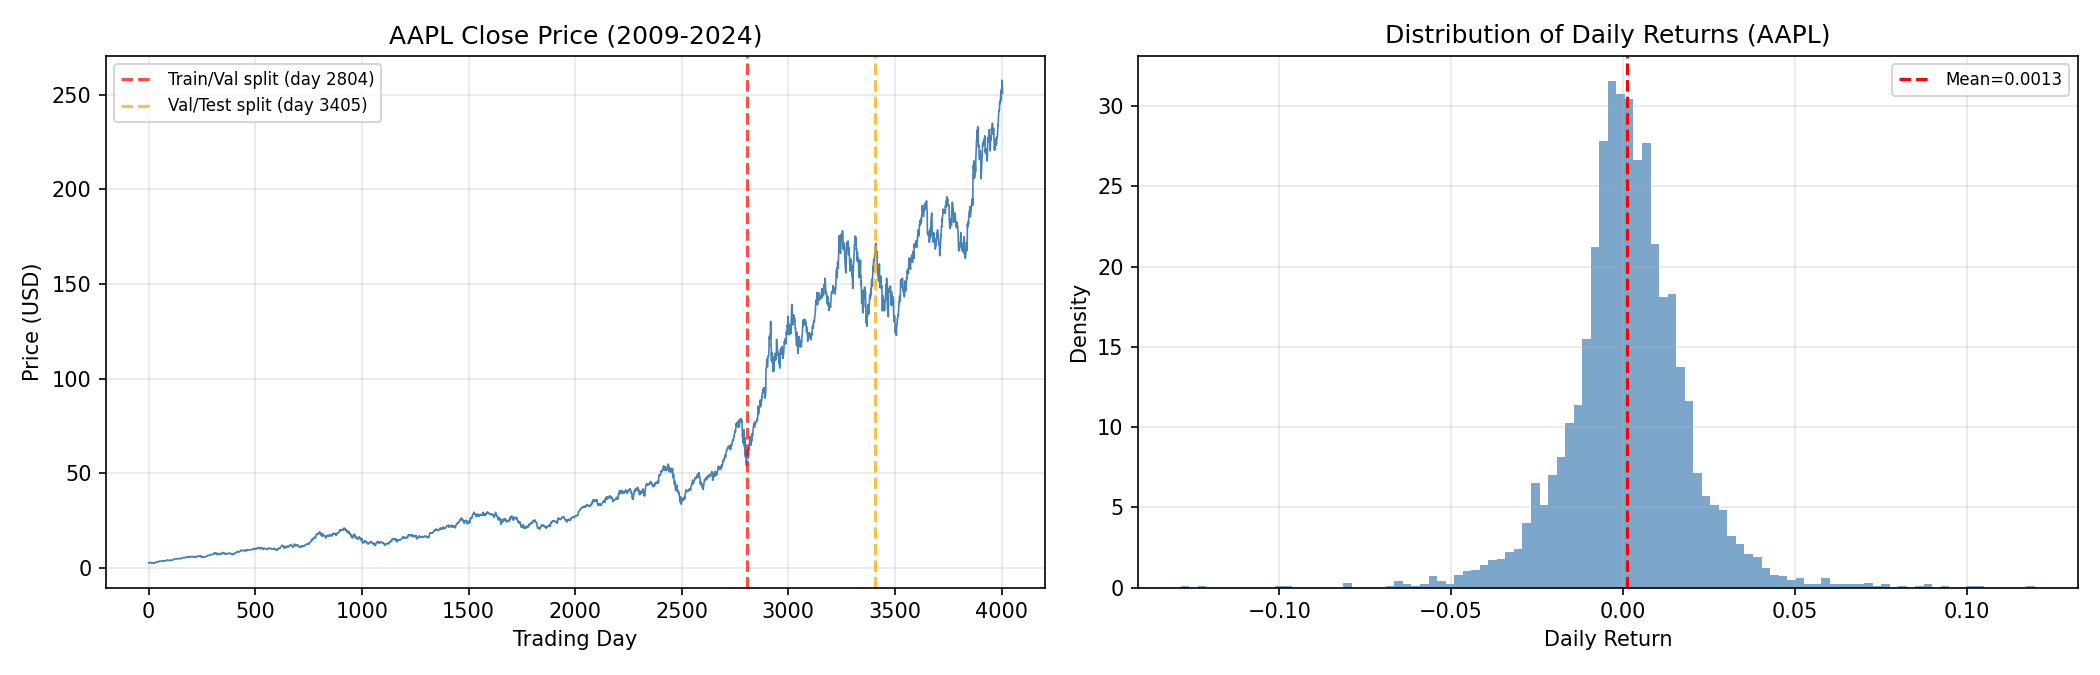
\includegraphics[width=0.95\textwidth]{results/data_exploration.png}
  \caption{Left: AAPL close price (2009--2024) with train/val/test boundaries. Right: Daily return distribution showing fat tails.}
  \label{fig:data}
\end{figure*}

%====================================================================
\section{Environment Design}
%====================================================================

We implement a Gym-style \texttt{TradingEnv} for single-asset trading.
The state $s_t \in \mathbb{R}^{10}$ consists of 9 normalised features plus the current position $\text{pos}_t \in \{-1, 0, +1\}$.
The agent chooses from three discrete actions: Sell ($-1$), Hold ($0$), Buy ($+1$).

The reward combines PnL, transaction costs, and a drawdown penalty:
\begin{multline}
  r_t = \text{pos}_t \cdot \tilde{r}_t
      - c_t \cdot \mathbf{1}[\text{pos}_t \neq \text{pos}_{t-1}] \\
      + \lambda \min\!\Bigl(0,\; \frac{V_t - V_t^{\text{peak}}}{V_t^{\text{peak}}}\Bigr)
  \label{eq:reward}
\end{multline}
where $\tilde{r}_t$ is the raw daily return, $\lambda = 0.5$, and $c_t$ is either a flat fee (10~bps) or proportional to position change magnitude.
The drawdown term encourages risk-averse behaviour.

Each episode spans one full data split. The environment tracks position history, trades, and portfolio value, and computes Sharpe ratio, max drawdown, and trade frequency at episode end.

%====================================================================
\section{Deep Learning Methods}
%====================================================================

\textbf{DQN} approximates $Q^*(s,a)$ with a neural network $Q_\theta$ trained via TD loss:
\begin{equation}
  \mathcal{L} = \mathbb{E}_{\mathcal{D}} \!\Big[\!
    \big( r + \gamma \max_{a'} Q_{\bar\theta}(s', a') - Q_\theta(s, a) \big)^2
  \Big]
  \label{eq:dqn}
\end{equation}
Key components (all from scratch): replay buffer (10K capacity, batch size 64), target network (updated every 100 steps), and linear $\varepsilon$-decay from 1.0 to 0.05 over 200K steps.

\textbf{DDQN} decouples action selection from evaluation to reduce overestimation:
\begin{equation}
  y_t = r + \gamma \, Q_{\bar\theta}\!\bigl(s',\; \arg\max_{a'} Q_\theta(s', a')\bigr)
  \label{eq:ddqn}
\end{equation}
DDQN subclasses DQN, changing only the target computation.

\textbf{Architecture.}
Both use a 3-layer MLP: $10 \to 128 \to 64 \to 3$ with ReLU activations, Adam ($\text{lr}{=}10^{-3}$), and gradient clipping (max norm 1.0).

%====================================================================
\section{Training and Results}
%====================================================================

Each agent trains for 200 episodes on the training set. Validation (greedy, $\varepsilon{=}0$) runs every 10 episodes. Both agents show clear learning, with DDQN converging slightly faster.

\begin{figure*}[t]
  \centering
  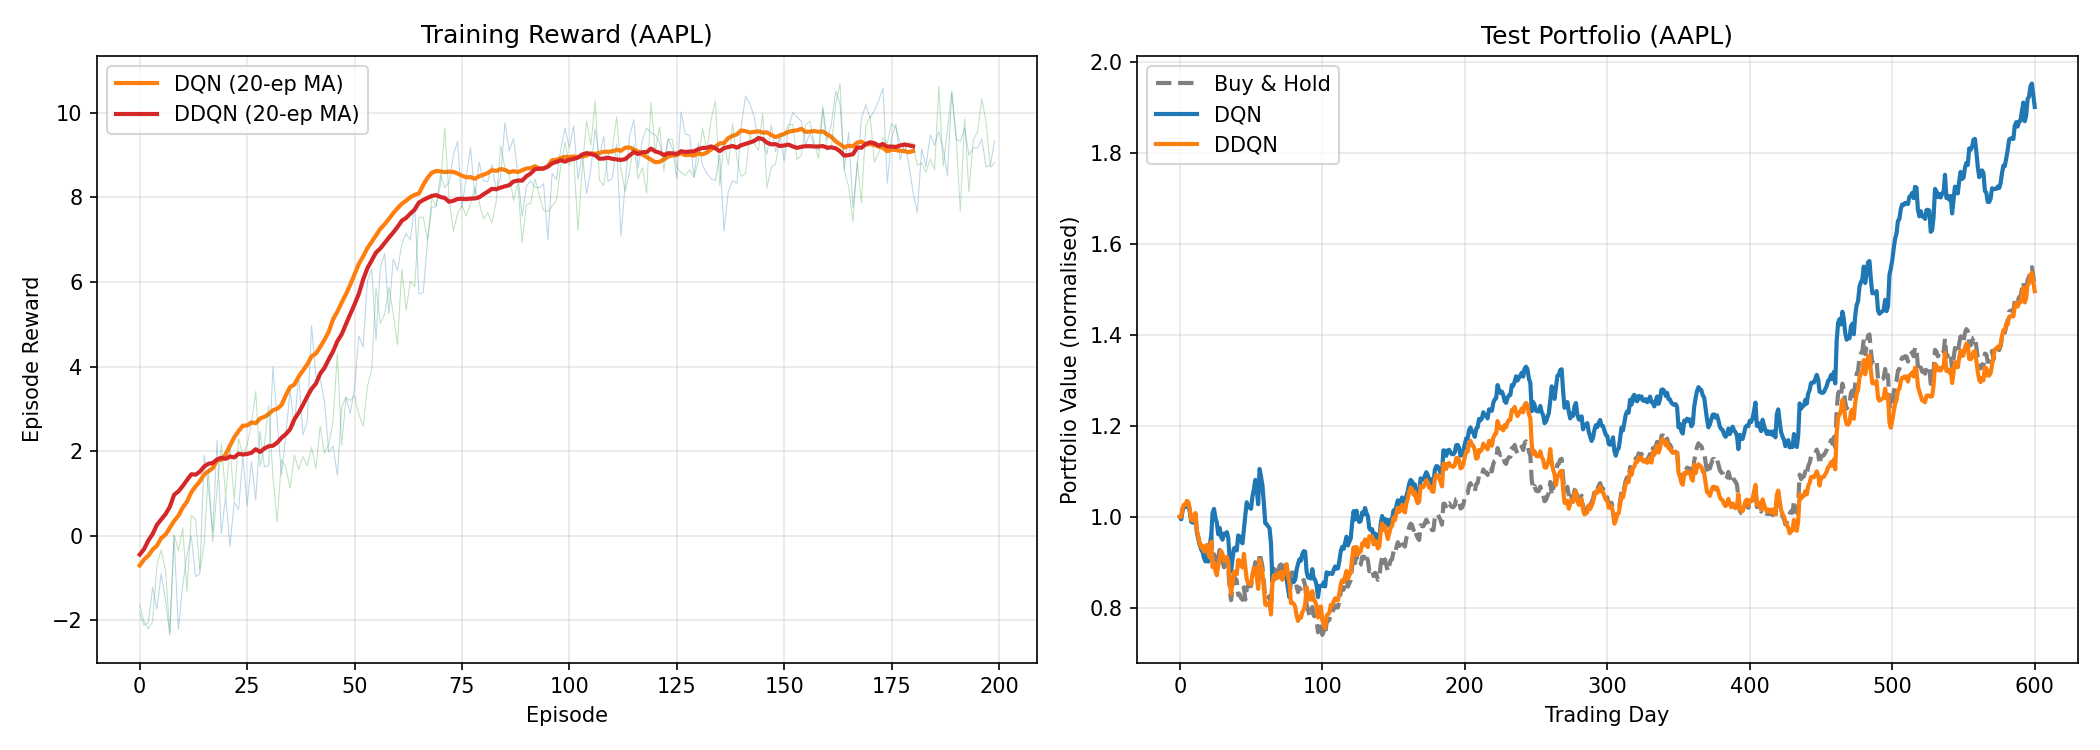
\includegraphics[width=0.95\textwidth]{results/results_AAPL.png}
  \caption{Left: Training reward (20-episode moving average). Right: Test portfolio value for DQN, DDQN, and buy-and-hold.}
  \label{fig:training}
\end{figure*}

\begin{table}[H]
\centering
\caption{Test performance on AAPL (601 days, 2022--2024).}
\label{tab:results}
\begin{tabular}{lccc}
\toprule
 & \textbf{DQN} & \textbf{DDQN} & \textbf{B\&H} \\
\midrule
Cum.\ Return   & +90.2\%   & +49.6\%   & +50.8\% \\
Sharpe          & 1.23      & 0.81      & 0.82    \\
Max DD          & $-$25.6\% & $-$27.1\% & $-$28.3\% \\
\bottomrule
\end{tabular}
\end{table}

DQN outperforms buy-and-hold on all metrics---higher return, better Sharpe, and lower drawdown---showing it learned to go flat or short during downturns and long during rallies.
DDQN matches buy-and-hold with slightly lower drawdown; its conservative Q-estimates reduce both upside and downside.
DQN's mild overestimation leads to more decisive positioning, which benefits when momentum signals are genuine.

%====================================================================
\section{Challenges}
%====================================================================

An early bug used normalised returns (std${\approx}1$) instead of raw returns for rewards, producing unrealistic values; fixed by separating \texttt{raw\_return}.
Exponential $\varepsilon$-decay exhausted exploration in one episode; linear decay over 200K steps resolved this.
Short-selling can cause portfolio values below zero, so we clamp at $10^{-8}$.

%====================================================================
\section{Future Work}
%====================================================================

Extensions include policy gradient methods (PPO) for continuous position sizing, multi-asset portfolio environments, LSTM architectures for temporal dependencies, and Sharpe/CVaR-based reward formulations.

%====================================================================
\section{Contributions}
%====================================================================

\begin{table}[H]
\centering
\small
\begin{tabular}{p{0.18\columnwidth} p{0.72\columnwidth}}
\toprule
\textbf{Member} & \textbf{Contributions} \\
\midrule
Rutwik &
DQN/DDQN implementation from scratch; hyperparameter tuning \\
\midrule
Yufan &
Data pipeline: \texttt{yfinance} OHLCV download, 9-feature engineering (RSI, MACD, Bollinger Bands, ATR, OBV, configurable MA deviations, volume normalisation), train-only z-score normalisation, multi-ticker \texttt{load\_all()} support.
\texttt{TradingEnv}: drawdown-penalised reward shaping (Eq.~\ref{eq:reward}), flat \& proportional transaction cost models, built-in Sharpe/drawdown/trade-frequency evaluation, position and portfolio tracking, episode logic \\
\midrule
Fei Xin &
Evaluation framework, training visualisation, report, and slides \\
\bottomrule
\end{tabular}
\end{table}

%====================================================================
\begin{thebibliography}{9}
\bibitem{mnih2015}
V.~Mnih et al., ``Human-level control through deep reinforcement learning,'' \emph{Nature}, 518:529--533, 2015.
\bibitem{hasselt2016}
H.~van Hasselt et al., ``Deep reinforcement learning with double Q-learning,'' \emph{AAAI}, 2016.
\bibitem{yang2020}
H.~Yang et al., ``Deep reinforcement learning for automated stock trading: An ensemble strategy,'' \emph{ACM ICAIF}, 2020.
\end{thebibliography}

\end{document}
